\chapter{\bf{State Diagram}}
\boldmath

\section{Input, Output e Stati}

Lo \textbf{state diagram} è una rappresentazione grafica che mostra i differenti stati in cui un sistema può trovarsi e le transizioni tra questi ultimi, in funzione di variabili esterne.

\vspace{3mm}

\noindent Gli input del diagramma principale sono:

\begin{itemize}
    \item \textbf{B1}: bottone per la chiusura e apertura del cancello
    \item \textbf{B2}: bottone per la regolazione del tempo di chiusura automatica del cancello
    \item \textbf{B3}: bottone per la regolazione del tempo di lavoro del cancello
    \item \textbf{P1}: sensore di presenza per la rilevazione di ostacoli
    \item \textbf{P2}: sensore di presenza per la rilevazione della chiusura completa del cancello
    \item $T_L$: timer relativo al tempo di lavoro
    \item $T_C$: timer relativo al tempo di chiusura automatica
    \item $T_E$: timer relativo al tempo di lavoro sommato ai 10 secondi di attesa per attendere l'attivazione del sensore $P2$
\end{itemize}

\noindent Gli output del diagramma sono:

\begin{itemize}
    \item \textbf{Led Green}
    \item \textbf{Led Yellow}
    \item \textbf{Led Red}
\end{itemize}

\noindent Gli stati del diagramma sono:

\begin{itemize}
    \item \textbf{Inattivo:} è lo stato iniziale del sistema, disponibile appena dopo l'accensione, durante il quale viene controllata l'attivazione dei due sensori di presenza $P1$ e $P2$ per garantire una corretta chiusura del cancello dopo l'accensione dello stesso;
    
    \item \textbf{Chiuso:} rappresenta lo stato per cui il cancello risulta completamente chiuso;
    
    \item \textbf{In Chiusura:} raffigura lo stato secondo cui il cancello si sta chiudendo, durante il quale si controlla l'eventuale presenza di ostacoli. Si controlla anche che il cancello si chiuda entro il tempo di lavoro ($T_L$) prestabilito; 
    
    \item \textbf{In Apertura:} delinea lo stato di apertura in corso del cancello, durante cui si controlla l'eventuale presenza di ostacoli;
    
    \item \textbf{Aperto:} rappresenta lo stato in cui il cancello risulta completamente aperto;
    
    \item \textbf{Aperto con Ostacolo:} descrive lo stato durante il quale il cancello è aperto ma è stata rilevata la presenza di un ostacolo dal sensore $P1$ e, dunque, non vi è possibilità di movimento;
    
    \item \textbf{Errore:} simboleggia lo stato di errore che si verifica nel momento in cui il cancello risulta non chiuso dopo il tempo prestabilito ($T_L$) più 10 secondi di attesa (i quali sommati formano il tempo di errore $T_E$).
\end{itemize}

\vspace{10mm}

\begin{figure}[H]
    \centering
    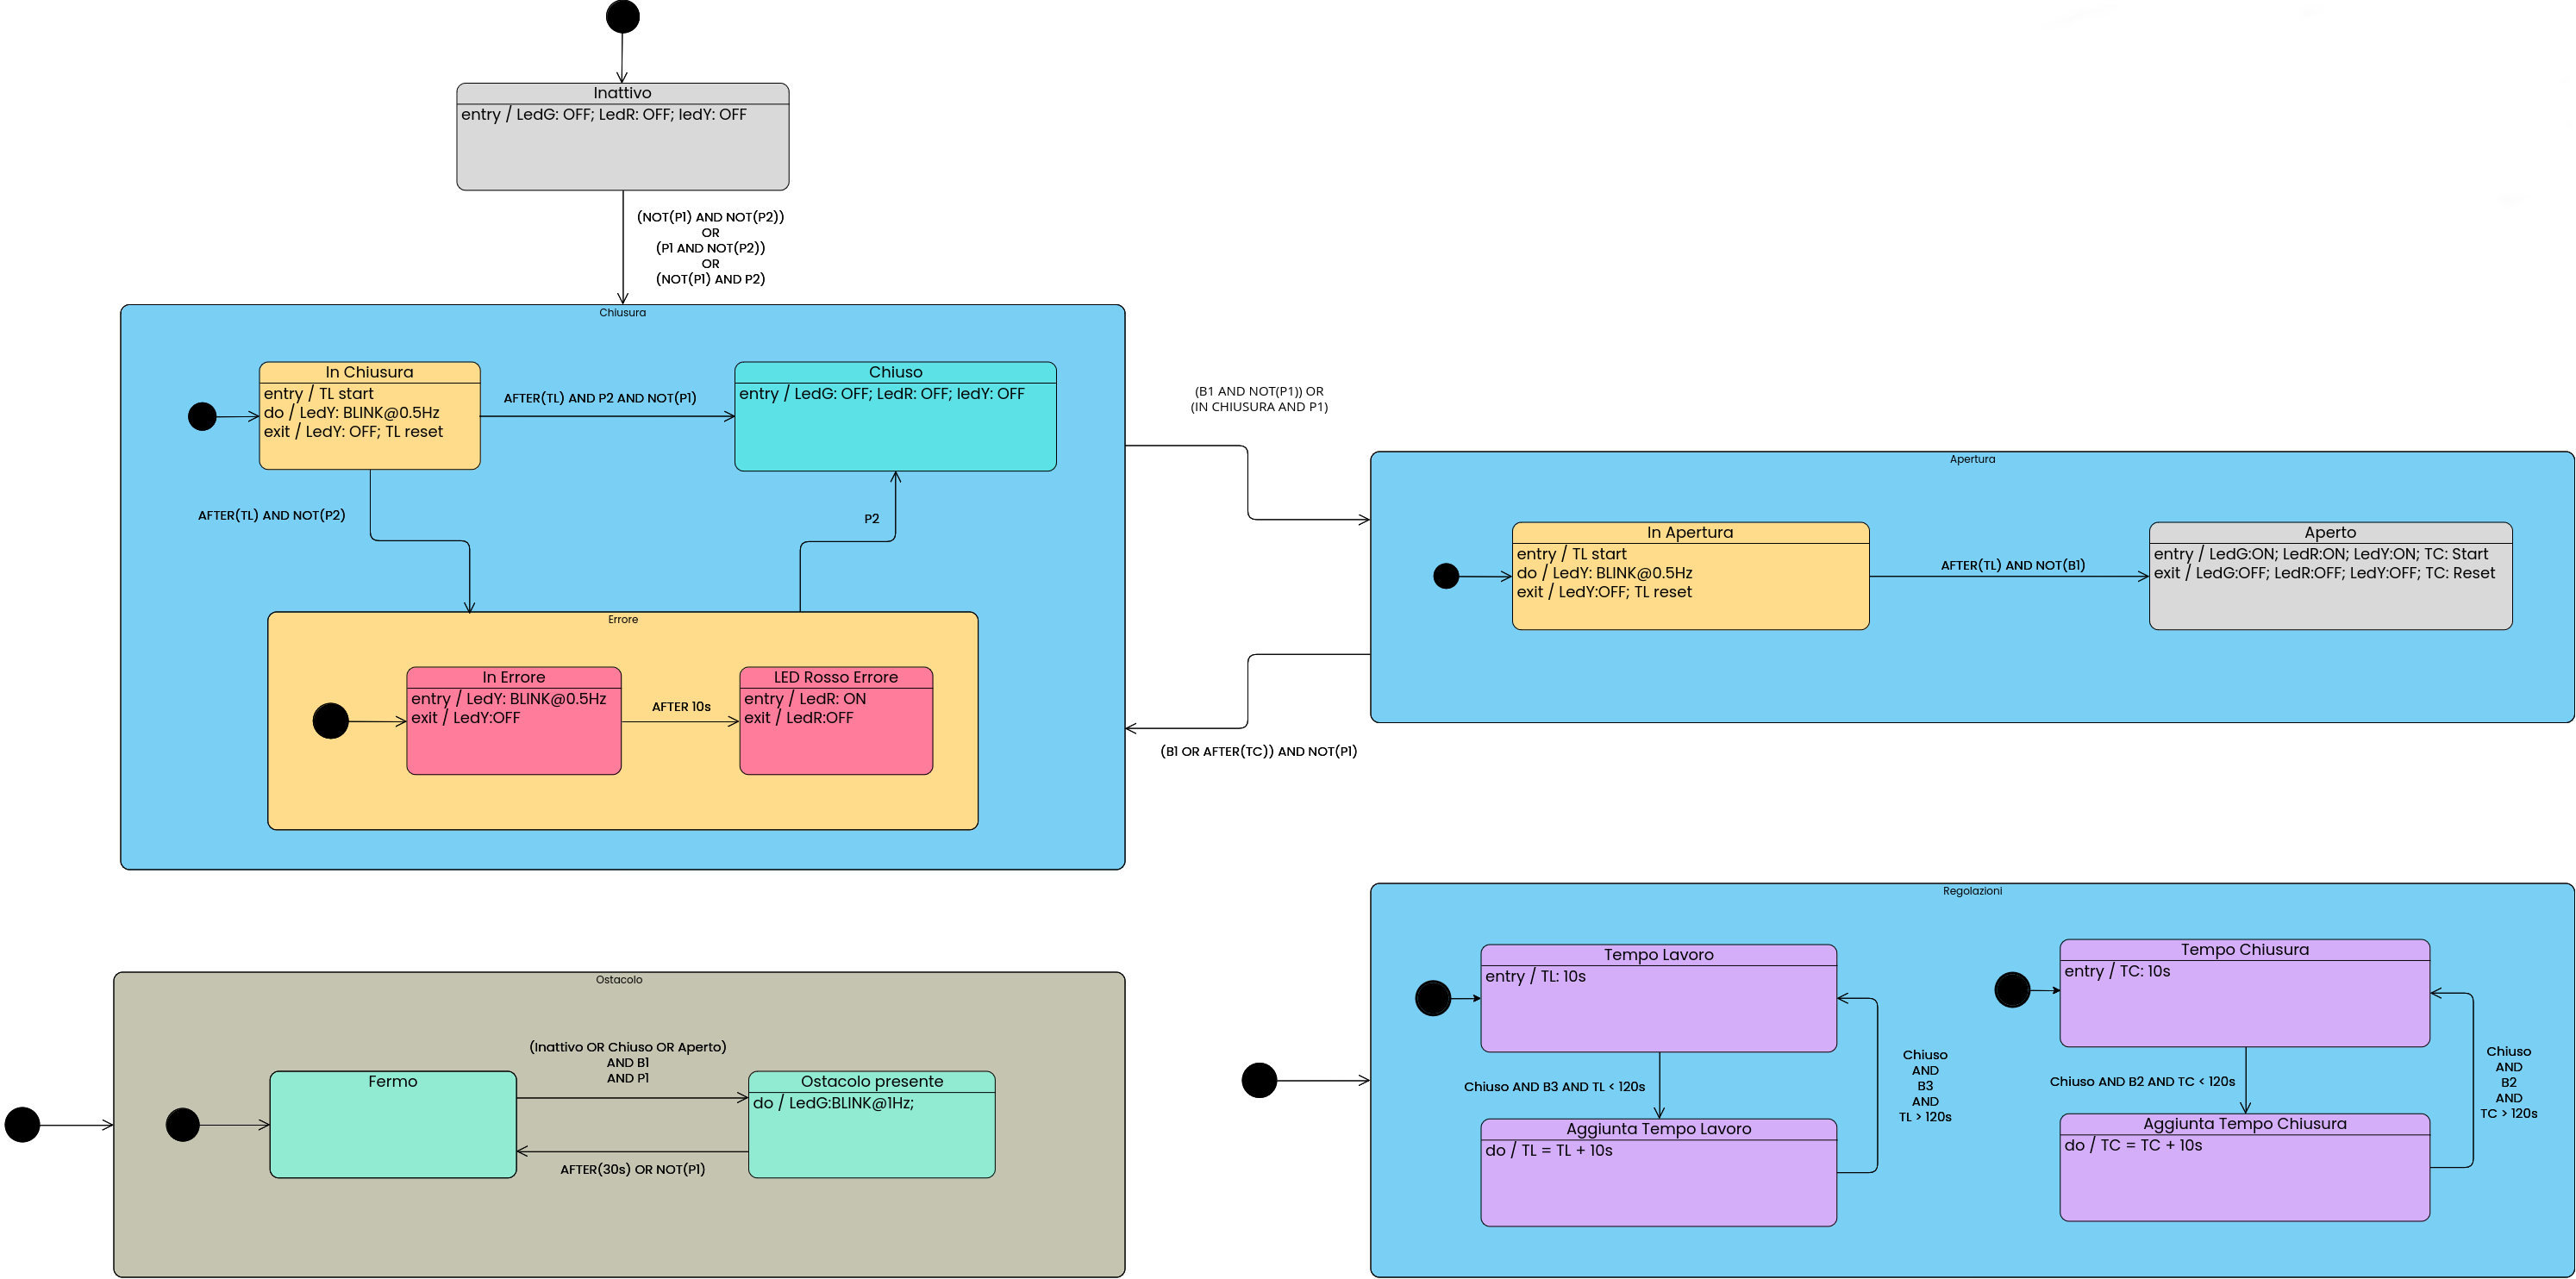
\includegraphics[width=0.9\textwidth]{figures/statediagram.png}
    \caption{State Diagram}
    \label{state}
\end{figure}


\section{Logica di Funzionamento}

\subsection{Stato \textit{Inattivo}}
All'avvio, il sistema si trova nello stato iniziale \textbf{Inattivo}, durante il quale si controlla lo stato dei due sensori di presenza $P1$ e $P2$, al fine di ritornare allo stato iniziale desiderato di \textbf{Cancello Chiuso}.

\noindent Le transizioni in uscita da esso sono:
\begin{itemize}
    \item Se è attivo il sensore di presenza $P1$, ma non il sensore $P2$, si rimane in questo stato in attesa che l'ostacolo venga rimosso;
    \item Se è attivo il sensore di presenza $P2$ si passa allo stato \textbf{Cancello Chiuso} per segnalarne la corretta chiusura;
    \item Se entrambi i sensori sono disattivati si procede alla chiusura passando allo stato \textbf{Cancello in Chiusura}.
\end{itemize}


\subsection{Stato \textit{Cancello Chiuso}}
In questo stato l'utente può regolare sia il tempo di lavoro ($T_L$) che il tempo di chiusura ($T_C$) tramite la pressione dei bottoni $B2$ e $B3$ in un range che va da 10 secondi a 120 secondi.

\noindent La transizione in uscita da questo stato è:
\begin{itemize}
    \item Se l'utente preme il bottone $B1$ si passa allo stato \textbf{Cancello in Apertura}.
\end{itemize} 

\noindent La pressione dei due bottoni $B2$ e $B3$ è ignorata in tutti gli altri stati.


\subsection{Stato \textit{Cancello in Apertura}}
In questo stato viene dapprima attivato il \textit{blink} del LED giallo per segnalare il movimento del cancello.

\noindent Le transizioni in uscita da questo stato sono:
\begin{itemize}
    \item Se l'utente preme il pulsante $B1$ si va nello stato \textbf{Cancello in Chiusura};
    \item Se dovesse scadere il tempo di lavoro ($T_L$) senza alcuna pressione del bottone $B1$ e senza alcun rilevamento di ostacoli, si entrerebbe nello stato \textbf{Aperto};
    \item Se dovesse scadere il tempo di lavoro ($T_L$), ma con rilevazione di ostacoli, si entrerebbe nello stato \textbf{Aperto con Ostacolo}.
\end{itemize}


\subsection{Stato \textit{Cancello in Chiusura}}
In questo stato viene dapprima attivato il \textit{blink} del LED giallo per segnalare il movimento del cancello.

\noindent Le transizioni in uscita da questo stato sono:
\begin{itemize}
    \item Se si attiva il sensore di presenza $P2$ si passa allo stato \textbf{Cancello Chiuso};
    \item Se l'utente preme il bottone $B1$ senza che vi sia la rilevazione di ostacoli o se viene rilevato un ostacolo senza la pressione del pulsante, si passa allo stato \textbf{Cancello in Apertura};
    \item Se dovesse scadere il tempo di errore ($T_E$), ma senza alcuna attivazione del sensore di presenza $P2$, si passerebbe allo stato di \textbf{Errore}.
\end{itemize}


\subsection{Stato \textit{Cancello Aperto}}
Nello stato in essere vengono accesi tutti i LED per segnalare la corretta apertura del cancello ed inoltre viene attivato anche il timer relativo alla chiusura ($T_C$).

\noindent Le transizioni in uscita da questo stato sono:
\begin{itemize}
    \item Se non è scaduto il timer $T_C$ e non viene rilevato nessun ostacolo, si rimane nello stato attuale;
    \item Se il timer $T_C$ scade e non viene segnalata la presenza di ostacoli, si passa allo stato \textbf{Cancello in Chiusura};
    \item Se il timer $T_C$ non scade, ma viene segnalata la presenza di ostacoli, si passa allo stato \textbf{Aperto con Ostacolo}.
\end{itemize}


\subsection{Stato \textit{Cancello Aperto con Ostacolo}}
In questo stato vengono spenti i LED giallo e rosso e viene fatto lampeggiare il LED verde per 30 secondi a partire dalla rilevazione dell'ostacolo.

\noindent Le transizioni in uscita dal sopracitato stato sono:
\begin{itemize}
    \item Se l'ostacolo è ancora presente ($P1$ ancora attivo) si rimane nello stato attuale;
    \item Se l'ostacolo non è più presente, si ritorna allo stato \textbf{Cancello Aperto}.
\end{itemize}


\subsection{Stato \textit{Errore}}
In questo stato viene acceso il LED rosso per segnalare lo stato di errore del cancello, causato dalla mancata chiusura dello stesso secondo il tempo prestabilito con l'aggiunta di 10 secondi di attesa($T_E$).

\noindent La transizione in uscita da esso è:
\begin{itemize}
    \item Se il sensore $P2$ si attiva, si passa allo stato \textbf{Cancello Chiuso}.
\end{itemize}